\begin{figure}[h]
    \centering



\tikzset{every picture/.style={line width=0.75pt}} %set default line width to 0.75pt        

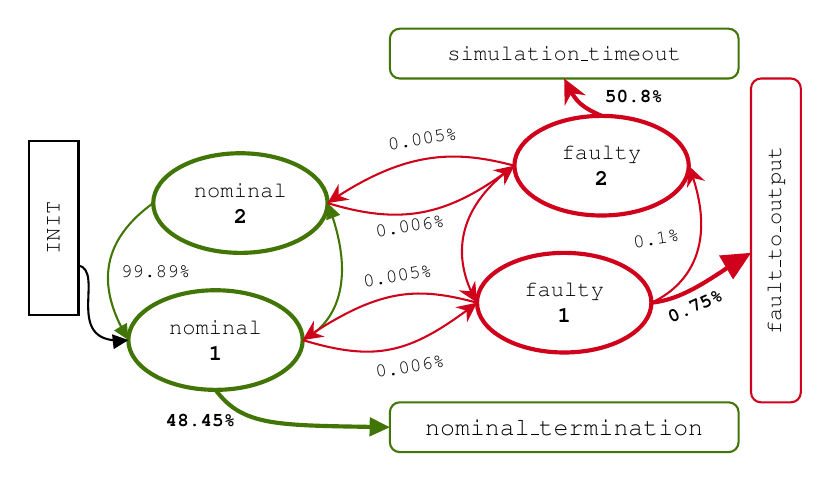
\begin{tikzpicture}[x=0.75pt,y=0.75pt,yscale=-1.2,xscale=1.2]
%uncomment if require: \path (0,300); %set diagram left start at 0, and has height of 300

%Rounded Diagonal Corner Rect [id:dp20075248017872083] 
\draw   (340,50) .. controls (340,50) and (340,50) .. (340,50) -- (360,50) .. controls (360,50) and (360,50) .. (360,50) -- (360,120) .. controls (360,120) and (360,120) .. (360,120) -- (340,120) .. controls (340,120) and (340,120) .. (340,120) -- cycle ;
%Shape: Ellipse [id:dp8528302096917133] 
\draw  [color={rgb, 255:red, 65; green, 117; blue, 5 }  ,draw opacity=1 ][fill={rgb, 255:red, 255; green, 255; blue, 255 }  ,fill opacity=0.28 ][line width=1.5]  (380,130) .. controls (380,118.95) and (395.67,110) .. (415,110) .. controls (434.33,110) and (450,118.95) .. (450,130) .. controls (450,141.05) and (434.33,150) .. (415,150) .. controls (395.67,150) and (380,141.05) .. (380,130) -- cycle ;
%Shape: Ellipse [id:dp18888957741575885] 
\draw  [color={rgb, 255:red, 208; green, 2; blue, 27 }  ,draw opacity=1 ][line width=1.5]  (535,60) .. controls (535,48.95) and (550.67,40) .. (570,40) .. controls (589.33,40) and (605,48.95) .. (605,60) .. controls (605,71.05) and (589.33,80) .. (570,80) .. controls (550.67,80) and (535,71.05) .. (535,60) -- cycle ;
%Rounded Rect [id:dp7596732624112932] 
\draw  [color={rgb, 255:red, 208; green, 2; blue, 27 }  ,draw opacity=1 ] (630,29) .. controls (630,26.79) and (631.79,25) .. (634,25) -- (646,25) .. controls (648.21,25) and (650,26.79) .. (650,29) -- (650,151) .. controls (650,153.21) and (648.21,155) .. (646,155) -- (634,155) .. controls (631.79,155) and (630,153.21) .. (630,151) -- cycle ;
%Curve Lines [id:da32583462836072785] 
\draw [color={rgb, 255:red, 208; green, 2; blue, 27 }  ,draw opacity=1 ][line width=1.5]    (626.45,97.16) .. controls (614.57,104.61) and (603.42,113.64) .. (590,115) ;
\draw [shift={(630,95)}, rotate = 149.68] [fill={rgb, 255:red, 208; green, 2; blue, 27 }  ,fill opacity=1 ][line width=0.08]  [draw opacity=0] (11.61,-5.58) -- (0,0) -- (11.61,5.58) -- cycle    ;
%Curve Lines [id:da3658243871665472] 
\draw    (376.92,130.2) .. controls (353.95,130.62) and (370.72,102.56) .. (360,100) ;
\draw [shift={(380,130)}, rotate = 173.77] [fill={rgb, 255:red, 0; green, 0; blue, 0 }  ][line width=0.08]  [draw opacity=0] (6.25,-3) -- (0,0) -- (6.25,3) -- cycle    ;
%Rounded Rect [id:dp11817172422118216] 
\draw  [color={rgb, 255:red, 65; green, 117; blue, 5 }  ,draw opacity=1 ] (621,155) .. controls (623.21,155) and (625,156.79) .. (625,159) -- (625,171) .. controls (625,173.21) and (623.21,175) .. (621,175) -- (489,175) .. controls (486.79,175) and (485,173.21) .. (485,171) -- (485,159) .. controls (485,156.79) and (486.79,155) .. (489,155) -- cycle ;
%Shape: Ellipse [id:dp43557254982651106] 
\draw  [color={rgb, 255:red, 65; green, 117; blue, 5 }  ,draw opacity=1 ][fill={rgb, 255:red, 255; green, 255; blue, 255 }  ,fill opacity=0.28 ][line width=1.5]  (390,75) .. controls (390,63.95) and (405.67,55) .. (425,55) .. controls (444.33,55) and (460,63.95) .. (460,75) .. controls (460,86.05) and (444.33,95) .. (425,95) .. controls (405.67,95) and (390,86.05) .. (390,75) -- cycle ;
%Shape: Ellipse [id:dp5343830480869827] 
\draw  [color={rgb, 255:red, 208; green, 2; blue, 27 }  ,draw opacity=1 ][line width=1.5]  (520,115) .. controls (520,103.95) and (535.67,95) .. (555,95) .. controls (574.33,95) and (590,103.95) .. (590,115) .. controls (590,126.05) and (574.33,135) .. (555,135) .. controls (535.67,135) and (520,126.05) .. (520,115) -- cycle ;
%Curve Lines [id:da2717718768343944] 
\draw [color={rgb, 255:red, 65; green, 117; blue, 5 }  ,draw opacity=1 ]   (450,130) .. controls (455.39,127.55) and (474.71,115.5) .. (460.89,77.37) ;
\draw [shift={(460,75)}, rotate = 428.82] [fill={rgb, 255:red, 65; green, 117; blue, 5 }  ,fill opacity=1 ][line width=0.08]  [draw opacity=0] (6.25,-3) -- (0,0) -- (6.25,3) -- cycle    ;
%Curve Lines [id:da23916036459047474] 
\draw [color={rgb, 255:red, 208; green, 2; blue, 27 }  ,draw opacity=1 ]   (590,115) .. controls (595.39,112.55) and (619.51,100.5) .. (605.88,62.37) ;
\draw [shift={(605,60)}, rotate = 428.82] [fill={rgb, 255:red, 208; green, 2; blue, 27 }  ,fill opacity=1 ][line width=0.08]  [draw opacity=0] (8.04,-3.86) -- (0,0) -- (8.04,3.86) -- (5.34,0) -- cycle    ;
%Curve Lines [id:da8274565221278805] 
\draw [color={rgb, 255:red, 208; green, 2; blue, 27 }  ,draw opacity=1 ]   (518.44,112.15) .. controls (511.34,98.05) and (509.91,78.08) .. (535,60) ;
\draw [shift={(520,115)}, rotate = 239.53] [fill={rgb, 255:red, 208; green, 2; blue, 27 }  ,fill opacity=1 ][line width=0.08]  [draw opacity=0] (8.04,-3.86) -- (0,0) -- (8.04,3.86) -- (5.34,0) -- cycle    ;
%Curve Lines [id:da4524486896686448] 
\draw [color={rgb, 255:red, 65; green, 117; blue, 5 }  ,draw opacity=1 ][line width=0.75]    (378.51,127.37) .. controls (370.77,113.26) and (364.78,93.17) .. (390,75) ;
\draw [shift={(380,130)}, rotate = 239.53] [fill={rgb, 255:red, 65; green, 117; blue, 5 }  ,fill opacity=1 ][line width=0.08]  [draw opacity=0] (6.25,-3) -- (0,0) -- (6.25,3) -- cycle    ;
%Curve Lines [id:da8065399762870671] 
\draw [color={rgb, 255:red, 208; green, 2; blue, 27 }  ,draw opacity=1 ]   (517.28,117.06) .. controls (492.7,135.43) and (479.11,138.85) .. (450,130) ;
\draw [shift={(520,115)}, rotate = 142.55] [fill={rgb, 255:red, 208; green, 2; blue, 27 }  ,fill opacity=1 ][line width=0.08]  [draw opacity=0] (8.04,-3.86) -- (0,0) -- (8.04,3.86) -- (5.34,0) -- cycle    ;
%Curve Lines [id:da3954387747286521] 
\draw [color={rgb, 255:red, 208; green, 2; blue, 27 }  ,draw opacity=1 ]   (532.26,62.06) .. controls (507.36,80.43) and (489.11,83.85) .. (460,75) ;
\draw [shift={(535,60)}, rotate = 142.55] [fill={rgb, 255:red, 208; green, 2; blue, 27 }  ,fill opacity=1 ][line width=0.08]  [draw opacity=0] (8.04,-3.86) -- (0,0) -- (8.04,3.86) -- (5.34,0) -- cycle    ;
%Curve Lines [id:da16071146130984038] 
\draw [color={rgb, 255:red, 208; green, 2; blue, 27 }  ,draw opacity=1 ]   (452.76,128.14) .. controls (482.07,108.67) and (496.88,108.86) .. (520,115) ;
\draw [shift={(450,130)}, rotate = 325.61] [fill={rgb, 255:red, 208; green, 2; blue, 27 }  ,fill opacity=1 ][line width=0.08]  [draw opacity=0] (8.04,-3.86) -- (0,0) -- (8.04,3.86) -- (5.34,0) -- cycle    ;
%Curve Lines [id:da2703895401851424] 
\draw [color={rgb, 255:red, 208; green, 2; blue, 27 }  ,draw opacity=1 ]   (462.78,73.14) .. controls (492.37,53.67) and (511.88,53.86) .. (535,60) ;
\draw [shift={(460,75)}, rotate = 325.61] [fill={rgb, 255:red, 208; green, 2; blue, 27 }  ,fill opacity=1 ][line width=0.08]  [draw opacity=0] (8.04,-3.86) -- (0,0) -- (8.04,3.86) -- (5.34,0) -- cycle    ;
%Curve Lines [id:da7497874187898392] 
\draw [color={rgb, 255:red, 65; green, 117; blue, 5 }  ,draw opacity=1 ][line width=1.5]    (480.42,164.92) .. controls (439.36,164.22) and (425.94,164.64) .. (415,150) ;
\draw [shift={(485,165)}, rotate = 181.07] [fill={rgb, 255:red, 65; green, 117; blue, 5 }  ,fill opacity=1 ][line width=0.08]  [draw opacity=0] (8.13,-3.9) -- (0,0) -- (8.13,3.9) -- cycle    ;
%Rounded Rect [id:dp7577300259636373] 
\draw  [color={rgb, 255:red, 65; green, 117; blue, 5 }  ,draw opacity=1 ] (621,5) .. controls (623.21,5) and (625,6.79) .. (625,9) -- (625,21) .. controls (625,23.21) and (623.21,25) .. (621,25) -- (489,25) .. controls (486.79,25) and (485,23.21) .. (485,21) -- (485,9) .. controls (485,6.79) and (486.79,5) .. (489,5) -- cycle ;
%Curve Lines [id:da08983874906696832] 
\draw [color={rgb, 255:red, 208; green, 2; blue, 27 }  ,draw opacity=1 ][line width=1.5]    (556.82,28.58) .. controls (559.85,34.34) and (561.83,36.34) .. (570,40) ;
\draw [shift={(555,25)}, rotate = 63.43] [fill={rgb, 255:red, 208; green, 2; blue, 27 }  ,fill opacity=1 ][line width=0.08]  [draw opacity=0] (9.91,-4.76) -- (0,0) -- (9.91,4.76) -- (6.58,0) -- cycle    ;

% Text Node
\draw (350,85) node  [font=\footnotesize,rotate=-270] [align=left] {{\fontfamily{pcr}\selectfont INIT}};
% Text Node
\draw (640,90) node  [font=\footnotesize,rotate=-270] [align=left] {{\fontfamily{pcr}\selectfont fault\_to\_output}};
% Text Node
\draw (555,165) node  [font=\footnotesize] [align=left] {{\fontfamily{pcr}\selectfont {\small nominal\_termination}}};
% Text Node
\draw (415,130) node  [font=\footnotesize] [align=left] {\begin{minipage}[lt]{37.003356000000004pt}\setlength\topsep{0pt}
\begin{center}
{\fontfamily{pcr}\selectfont nominal}\\{\fontfamily{pcr}\selectfont \textbf{1}}
\end{center}

\end{minipage}};
% Text Node
\draw (570,60) node  [font=\footnotesize] [align=left] {\begin{minipage}[lt]{32.101644pt}\setlength\topsep{0pt}
\begin{center}
{\fontfamily{pcr}\selectfont faulty}\\{\fontfamily{pcr}\selectfont \textbf{2}}
\end{center}

\end{minipage}};
% Text Node
\draw (425,75) node  [font=\footnotesize] [align=left] {\begin{minipage}[lt]{37.003356000000004pt}\setlength\topsep{0pt}
\begin{center}
{\fontfamily{pcr}\selectfont nominal}\\{\fontfamily{pcr}\selectfont \textbf{2}}
\end{center}

\end{minipage}};
% Text Node
\draw (555,115) node  [font=\footnotesize] [align=left] {\begin{minipage}[lt]{32.101644pt}\setlength\topsep{0pt}
\begin{center}
{\fontfamily{pcr}\selectfont faulty}\\{\fontfamily{pcr}\selectfont \textbf{1}}
\end{center}

\end{minipage}};
% Text Node
\draw (555,15) node  [font=\footnotesize] [align=left] {{\fontfamily{pcr}\selectfont simulation\_timeout}};
% Text Node
\draw (391,102.5) node  [font=\scriptsize] [align=left] {{\fontfamily{pcr}\selectfont 99.89\%}};
% Text Node
\draw (498.08,49.3) node  [font=\scriptsize,rotate=-350.99] [align=left] {{\fontfamily{pcr}\selectfont 0.005\%}};
% Text Node
\draw (493.08,84.3) node  [font=\scriptsize,rotate=-350.99] [align=left] {{\fontfamily{pcr}\selectfont 0.006\%}};
% Text Node
\draw (591.92,89.3) node  [font=\scriptsize,rotate=-350.99] [align=left] {{\fontfamily{pcr}\selectfont 0.1\%}};
% Text Node
\draw (493.08,140.7) node  [font=\scriptsize,rotate=-350.99] [align=left] {{\fontfamily{pcr}\selectfont 0.006\%}};
% Text Node
\draw (488.08,104.3) node  [font=\scriptsize,rotate=-350.99] [align=left] {{\fontfamily{pcr}\selectfont 0.005\%}};
% Text Node
\draw (583,32.5) node  [font=\scriptsize] [align=left] {{\fontfamily{pcr}\selectfont \textbf{50.8\%}}};
% Text Node
\draw (607.64,116.42) node  [font=\scriptsize,rotate=-335.61] [align=left] {{\fontfamily{pcr}\selectfont \textbf{0.75\%}}};
% Text Node
\draw (409,162.5) node  [font=\scriptsize] [align=left] {{\fontfamily{pcr}\selectfont \textbf{48.45\%}}};


\end{tikzpicture}
    \caption{Extracted FSM for the I2C Block}
    \label{fig:simp_fsm}
\end{figure} 
